\section{Deep Neural Networks}

In this section, we will talk about some recent extension version of DNN models which
actually comes form the generalization of convolutional neural networks.

First, the so-called one hidden layer neural networks can be defined by
\begin{equation}
DNN_1=span\{\sigma(wx+b), w\in\mathbb{R}^n ,b\in\mathbb{R} \}
\end{equation}
with
$$
\theta(x) = wx+b \in\mathbb{R}^m, w=(w_i,\cdots,w_m)^T,\ w_i\in\mathbb{R}^{1\times n}
$$	
and
\begin{equation*}
\theta(x) = 	wx+b=\left(\begin{array}{c}
		w_1x+b \\ 
		\vdots \\ 
		w_m x+b_m
	\end{array} 
	\right)
\end{equation*}
Let $\sigma$ be the activation function, say Heaviside, sigmoid, $\tanh x$, ReLU. The deep neural network is defined as 
\begin{equation*}
	\begin{aligned}
		&x^0 = x,\\
		&f^{n+1}=\sigma(w^n x^n+b^n)=(\sigma\circ\theta)(f^n)\\
		&DNN_i = \{w^i f^i +b^i \}
	\end{aligned}
\end{equation*}
Then we have
\begin{equation}
  \label{eq:1}
DNN_{i+1} = \{\theta(f^{i+1}) \}
=\{\theta(\sigma\circ\theta)(f^i) \}
=(\theta\circ\sigma) DNN_{i} 
\end{equation}
and $\#$ of layers = $\#$ of $\sigma$ applied.


More general DNN:
\begin{equation}
	\begin{aligned}
		DNN_0&=\{wx+b\}\\
		DNN_J&=\{(\theta\circ\sigma)\circ f_{J-1}, \ f_{J-1}\in DNN_{J-1}\}
	\end{aligned}
\end{equation}
DNN contains ResNet, iResNet, DenseNet, MgNet.

The question is whether $DNN_k\subset DNN_{k+1}$ is true. The answer is that $DNN_k\subset DNN_{k+1}$ is only true for the case that the activation function is ReLU, since $x=ReLU(x)-ReLU(-x)$.

\chapter{The Sparse Grid Method}
It is well-known that a smooth function defined on $[0,1]^d$
can be pointwisely approximated with $O(h^2)$ accuracy by
a piecewise bilinear function in a subspace $V_h$ of dimension $O(h^{-d})$.
In the socalled sparse grid method proposed by
Zenger \cite{zenger1990sparse}, an $O(h^2|\log h|^{d-1})$ pointwise
accuracy can be achieved by using a  substantially smaller
subspace $S_h\subset V_h$ of dimension $O(h^{-1}|\log h|^{d-1})$.
As a result, a function $u$ on a general domain in $\R^d$
can be approximated with $O(h|\log h|^{d-1})$ in $H^1$ norm
with only $O(h^{-1}|\log h|^{d-1})$ number of operations.

\section{Multi-linear finite elements}

For simplicity, we take
$$
D_s=(0,1)^s,\ 1\leq s\leq d.
$$
For $D_1$, let the first grid $\mathcal{T}_0^1$ be itself, namely $\mathcal T_0^1=\{(0, 1)\}$. Divide each
element of $\mathcal{T}_k^1$ into two equal intervals and obtain the
next level grid $\mathcal{T}_{k+1}^1$ . For $s=1$, denote the basis function of nodal value interpolation to the vertex $x_{k,i}=ih_k$ by $\phi_{k,i}(x)$ with $0\leq i\leq n_k$.   
\begin{figure}[!ht]
\begin{center}
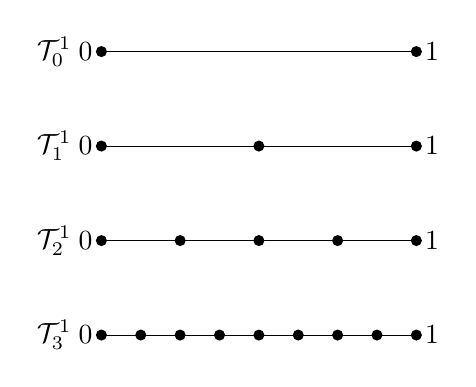
\begin{tikzpicture}[xscale=4,yscale=4]
\draw[-] (0,0.9) -- (1,0.9);
\draw[-] (0,0) -- (1,0);
\draw[-] (0,0.3) -- (1,0.3);
\draw[-] (0,0.6) -- (1,0.6);
\fill(0,0.9) circle(0.5pt);
\fill(1,0.9) circle(0.5pt);

\fill(0,0.6) circle(0.5pt);
\fill(0.5,0.6) circle(0.5pt);
\fill(1,0.6) circle(0.5pt);

\fill(0,0.3) circle(0.5pt);
\fill(0.25,0.3) circle(0.5pt);
\fill(0.5,0.3) circle(0.5pt);
\fill(0.75,0.3) circle(0.5pt);
\fill(1,0.3) circle(0.5pt);

\fill(0,0) circle(0.5pt);
\fill(0.125,0) circle(0.5pt);
\fill(0.25,0) circle(0.5pt);
\fill(0.375,0) circle(0.5pt);
\fill(0.5,0) circle(0.5pt);
\fill(0.625,0) circle(0.5pt);
\fill(0.75,0) circle(0.5pt);
\fill(0.875,0) circle(0.5pt);
\fill(1,0) circle(0.5pt);

\node at (-0.15,0) {$\mathcal{T}_3^1$};
\node at (-0.15,0.3) {$\mathcal{T}_2^1$};
\node at (-0.15,0.6) {$\mathcal{T}_1^1$};
\node at (-0.15,0.9) {$\mathcal{T}_0^1$};
\node at (-0.05,0) {$0$};
\node at (-0.05,0.3) {$0$};
\node at (-0.05,0.6) {$0$};
\node at (-0.05,0.9) {$0$};
\node at (1.05,0.9) {$1$};
\node at (1.05,0) {$1$};
\node at (1.05,0.3) {$1$};
\node at (1.05,0.6) {$1$};
\end{tikzpicture}
\end{center}
\end{figure}

Consider a cubic grid $
\mathcal{T}_k^s$ of the domain $D_s$, which is a tensor product of
$\mathcal{T}_k^1$. The vertice of elements there are $(i_1h_k, \cdots
, i_s h_k)$, with $0\leq i_1, \cdots, i_s\leq n_k$, $n_k=h_k^{-1}$
and $h_k=2^k$. For $1\leq s\leq d$, let
$$
\textbf{i}=(i_1,\cdots,i_s) \text{ and } x_{k,\textbf{i}}=(i_1h_k,\cdots, i_sh_k)
$$
and $\psi_{k, \textbf{i}}^s (x_1,\cdots,x_s)$ be the basis function of the nodal value interpolation(bilinear interpolation) corresponding to the vertex $(i_1h_k, \cdots , i_s h_k)$ on the grid $\mathcal{V}_k$. Then
\begin{equation}
\psi_{k, \textbf{i}}^s(x)=\prod_{j=1}^s\phi_{k,i_j}^j(x_j),
\quad 0\le i_j\le n_k,\quad 1\le s\le d.
\end{equation}
Here we add a superscript $j$ to each basis function $\phi_{k,i_j}$ to represent that the corresponding function is the basis function with respect to $x_j$ of $x=(x_1,\cdots,x_s)$. In other words, the grid $\mathcal{T}_k^s$ is obtained by cutting each cubic of $\mathcal{T}_{k-1}^s$ into $2^s$ equal cubics. Then the number of elements in $\mathcal{T}_k^s$ is $(n_k)^s=2^{ks}$ and the number of interior nodes is $(n_k-1)^s=(2^k-1)^s$.

\begin{lemma}\Label{lm:1}
Assume that $\Pi_k^s: C(\bar D_s)\mapsto \mathcal{T}_k^s(D_s)$ is the nodal value interpolant on $\mathcal{T}_k$ and $I_k^s$ is the nodal value interpolant with respect to the variable $x_s$.  Then
%: C(\bar D_1)\mapsto \mathcal{T}_k^s(D_1)
$$\Pi_k^d u=\prod_{s=1}^d I^s_k u.$$
\end{lemma}
\begin{proof}
For each $1\leq s\leq d$, let
$$
\mathcal{I}_k^s=\{\textbf{i}=(i_1,\cdots,i_s),\ 0\leq i_1,\cdots ,i_s\leq n_k\}.
$$
\begin{equation}
\begin{split}
\Pi_k^d u&= \sum_{\textbf{i}\in \mathcal{I}_k^d} u(x_{k,\textbf{i}}) \psi_{k,\textbf{i}}^d\\
&= \sum_{\textbf{i}\in \mathcal{I}_k^d} u(x_{k,\textbf{i}})  \prod_{s=1}^d\phi_{k,i_s}^s(x_s)\\
&= \sum_{\textbf{i}\in \mathcal{I}_k^d}  \prod_{s=1}^{d-1}\phi_{i_s}^s(x_{s})\sum_{1\leq i_d\leq n_k-1} u(x_{k,\textbf{i}})\phi_{i_d}^d(x_d)\\
&=\sum_{\textbf{i}\in \mathcal{I}_k^{d-1}}  \prod_{s=1}^{d-1}\phi_{i_s}^s(x_{s})  (I_k^d u)(x_{k,\textbf{i}}) \\
&=(\prod_{s=1}^d I_k^s) u.
\end{split}
\end{equation}
\end{proof}
\input{3FEM/1DHBasis}

From this one dimensional hierarchical basis, a multi-dimensional discrete space on the $d$-dimensional unite cube $D_d$ is obtain by a tensor product construction:
\begin{equation}
\begin{aligned}
\m_J^d &= \otimes_{s=1}^d \m_J\\%\overbrace{\m_J\otimes \m_J\otimes \cdots \otimes \m_J}^{d}\\
&= \bigoplus_{k_1,k_2,\cdots k_d=0}^J  \otimes_{s=1}^d V_{k_s}^s%( \mathcal V_{k_1}^1 \otimes  \mathcal V_{k_2}^2\otimes\cdots \otimes  \mathcal V_{k_d}^d)\\
&= \bigoplus_{j=0}^{dJ}\bigoplus_{k_1+k_2+\cdots + k_d= j}  \otimes_{s=1}^d V_{k_s}^s.%( \mathcal V_{k_1}^1 \otimes  \mathcal V_{k_2}^2\otimes\cdots \otimes  \mathcal V_{k_d}^d).
\end{aligned}
\end{equation}
Here the superscript $i$ of $V_{k_i}^i$ represents that this is the subspace for the $i$-th coordinate space.
Let $\mathbf{k}=(k_1,k_2,\cdots,k_d)$ be a multi-index. Denote
$$
\mathcal V_{\mathbf{k}} = \mathcal V_{k_1}^1 \otimes  \mathcal V_{k_2}^2\otimes\cdots \otimes  \mathcal V_{k_d}^d.
$$
The discrete space $\m_J^d$ can be written as 
\begin{equation}
\begin{aligned}
\m_J^d &= \bigoplus_{|\mathbf{k}|_\infty=J} \mathcal V_{\mathbf{k}} \\
&= \bigoplus_{j=0}^{dJ}\bigoplus_{|\mathbf{k}|_1=j} \mathcal V_{\mathbf{k}}.
\end{aligned}
\end{equation}
Let 
$$
\mathbf{I_l}=\{\mathbf{i}\in \mathbb{N}^d: \mathbf{1}\le \mathbf{i}\le 2^\mathbf{l}-1, i_j \text{ is odd for all }1\le j\le d\},
$$
and the hierarchical basis 
$$
\{\psi_\mathbf{k, i}^d: \mathbf{i}\in \mathbf{I_k}, \mathbf{k}\le \mathbf{l}\}\quad \mbox{with}\quad \psi_\mathbf{k, i}=\Pi_{s=1}^d\phi_{k_s,x_s}^s.
$$
For the $d$-dimensional hierarchical basis functions with $d\neq 2$, it is often more convenient to use the scaled HB
(hierarchical basis)
as follows
\begin{equation}
\label{shb}
\{\psi_\mathbf{k, i} \in {\cal V}_{\mathbf{k}}: \psi_\mathbf{k, i}=2^{-(|\mathbf{k}|_1+d)}\psi_{ \textbf{k, i}}^d, |\mathbf{k}|_\infty\le J\}. 
\end{equation}
With a proper ordering, we shall denote the scaled HB by $\{\psi_i,
i=1:N\}$. The HB in multiple dimensions is formally a direct generalization of the
HB in the one dimensional case.  But the property for the corresponding
stiffness matrix in multiple dimensions is not at all as clear as in one
dimension where the stiffness matrix is an identity matrix in some
special cases.  In this section, we shall show that at least in two
dimensions, a hierarchical basis is still very useful.




For the linear finite element,
$
\|u-u_I\|_0\lesssim h^2|u|_2.
$
Since $h\approx N^{-1/d}$, where $N$ is the number of the total degree of freedom, we have
$$
\|u-u_I\|_0\lesssim N^{-2/d}|u|_2.
$$
It implies that for a fixed number of degrees of freedom $N$, a large dimension results in pretty low accuracy.

In order to overcome the curse of dimensionality, we intend to choose a small subspace properly and throw away a large number of useless information. In the following, we introduce an interpolation operator $R_h$ which interpolates functions into finite element spaces on coarse meshes. Denote the range of $R_k^d$ by $S_k^d$, which is the desirable subspace.

Next we consider the approximation property and dimension  of the following subspace:
$$
S_{J,r}^d = \bigoplus_{|\mathbf{k}|_1 \le r}\mathcal V_{\mathbf{k}}.
$$
Denote
$$
\mathcal F_{J,r}=\{\mathbf k=(k_1,\cdots,k_d): 0\leq k_i\leq J, \ |\mathbf k|_1\leq r\},
$$
$$
\mathcal F_{J,r}^c=\{\mathbf k=(k_1,\cdots,k_d): 0\leq k_i\leq J, \ |\mathbf k|_1> r\},
$$
$$
\mathcal F_{J,r}^o=\{\mathbf k=(k_1,\cdots,k_d): 0\leq k_i\leq J, \ |\mathbf k|_1= r\}.
$$


%Next, we discuss the number $2^{-(2-m)r}\#\  \mathcal F_{J,r}^o$.
%\begin{enumerate}
%\item $r\leq J$: $\# \ \mathcal F_{J,r}^o=\#\ \{\mathbf k:  |\mathbf k|_1= r\}=C_{r+d-1}^r$. In this case, $r$ is usually small, we have
%$$
%\# \ \mathcal F_{J,r}^o= \frac{d(d+1)\cdots (d+r-1)}{r!}\approx d^r,\ \text{ and }2^{-(2-m)r}\#\  \mathcal F_{J,r}^o\approx 2^{-(2-m)r}d^r;
%$$
%\item $J<r\leq Jd$: For 2 dimensional case, let $k_i=a_i^2$, $r=r_0^2$. Then 
%$$
%\#\  \mathcal F_{J,r}^o=\# \{\mathbf{a}=(a_1,\cdots,a_d): \sum_{i=1}^da_i^2=r_0^2,\ 0\leq a_i\leq \sqrt{J}\}.
%$$
%We consider the length $l_\theta=r_0(2 \theta-\frac{\pi}{2})$ with $r_0\sin \theta=\sqrt{J}$. Then 
%$$
%l_\theta=\frac{\sqrt{J}}{\sin \theta}(2 \theta-\frac{\pi}{2}).
%$$
%A simple computation gives
%$$
%\sin \theta l_\theta'+\cos \theta l_\theta=2\sqrt{J},
%$$
%thus,
%$$
%\sin \theta l_\theta=\frac{\pi\sqrt{J}}{2} -2\sqrt{J}(\frac{\pi}{2}-\theta)=2\sqrt{J}(\theta-\frac{\pi}{4}),
%$$
%namely $l_\theta= 2\sqrt{J}(\theta-\frac{\pi}{4})/\sin \theta$. As $r$ grows larger, $l_\theta$ approximates $2\sqrt{J}$.
%
%\item $r> Jd$: $\# \ \mathcal F_{J,r}^o=0$.
%\end{enumerate}

\begin{lemma}\Label{lm:2}
Assume that
$I^s_k: C(\bar D)\mapsto \m_l(D_1)$ is the nodal value interpolant
with respect to the variable $x_s$.  Define
$$
F_{J,r}^d=\sum_{\mathbf k\in \mathcal{F}_{J,r}}\prod_{s=1}^d(I^s_{k_s}-I^s_{k_{s}-1})
$$
and
$$
S_{J,r}^d=F_{J,r}^d\m.
$$
Then for $m=0,1$,
$$
\inf_{\chi\in S_{J,r}^d}\nm{v-\chi}{m, D_d}\le C h_J^{(2-m)(r+1)/J}|\log h_J|^{d-1}\max_{|\mathbf k|_1> r}\nm {\partial^{2\text{sign}(\mathbf k)}v}{0,D_d}.
$$
\end{lemma}
\begin{proof}
Using the obvious identity (with $I_{-1}^s=0$)
$$I^s_J=\sum_{k=0}^J(I^s_k-I^s_{k-1}),$$
it follows from the commutative property and Lemma \ref{lm:1} that
$$
\Pi_J^d=\prod_{s=1}^d\sum_{k=0}^J(I^s_{k}-I^s_{k-1})
=\sum_{k_1,k_2,\cdots, k_d=0}^J\prod_{s=1}^d(I^s_{k_s}-I^s_{k_s-1}). 
$$
Thus,
\begin{equation}\label{multiNote1}
(\Pi_J^d-F_{J,r}^d)v=
\sum_{\mathbf k\in \mathcal{F}_{J,r}^c}\prod_{s=1}^d(I^s_{k_s}-I^s_{k_s-1})v.
\end{equation}
Note that if $k_1\neq 0$ and $m\le 2$,
\begin{equation}\label{multiNote201}
\begin{split}
\nm { \prod_{s=1}^d(I^s_{k_s}-I^s_{k_s-1})v}{m,D_d}
&\lesssim h^{2-m}_{k_1}\nm {\partial^2_{x_1}\prod_{s=2}^d(I^s_{k_s}-I^s_{k_s-1})v}{0, D_d} \\
&=  h^{2-m}_{k_1}\nm {\prod_{s=2}^d(I^s_{k_s}-I^s_{k_s-1}) \partial^2_{x_1} v}{0, D_d} \\
&=2^{-k_1(2-m)}\nm {\prod_{s=2}^d(I^s_{k_s}-I^s_{k_s-1}) \partial^2_{x_1} v}{0, D_d}.
%&\lesssim  h^{2-m}_{k_1}h^{2-m}_{k_2}\nm {\prod_{s=3}^d(I^s_{k_s}-I^s_{k_s-1}) \partial^2_{x_1} v}{L^{p}(D_d)} \\
%&\le Ch^{2-m}_{k_1}h^{2-m}_{k_2}\cdots h^{2-m}_{k_d}
%\nm{\partial^2_{x_1}\partial^2_{x_2}\cdots \partial^2_{x_d}v}{L^p(D_d)}.
\end{split}
\end{equation}
If $k_1=0$ and $m\le 2$,
\begin{equation}\label{multiNote202}
\begin{split}
\nm { \prod_{s=1}^d(I^s_{k_s}-I^s_{k_s-1})v}{m,D_d}
&= \nm { I_0^1 \prod_{s=2}^d(I^s_{k_s}-I^s_{k_s-1})v}{m,D_d} \\ 
&=2^{-k_1(2-m)}\nm {\prod_{s=2}^d(I^s_{k_s}-I^s_{k_s-1})  I_0^1  v}{m,D_d}.
\end{split}
\end{equation}
A combination of \eqref{multiNote201} and \eqref{multiNote202} gives
\begin{equation}\label{multiNote2}
\nm {\prod_{s=1}^d(I^s_{k_s}-I^s_{k_s-1})v}{0, D_d} 
\lesssim 2^{-(2-m)|\mathbf k |_1}\nm {\partial^{2\text{sign}(\mathbf k)}v}{0,D_d}.
\end{equation}
An elementary calculation shows that
\begin{equation}\label{multiNote3}
\begin{split}
\sum_{\mathbf k\in \mathcal{F}_{J,r}^c}2^{-(2-m)|\mathbf k |_1}\nm {\partial^{2\text{sign}(\mathbf k)}v}{0,D_d}
&=\sum_{j=r+1}^{Jd}\sum_{\mathbf k \in \mathcal F_{J,j}^o}2^{-(2-m)|\mathbf k |_1}\nm {\partial^{2\text{sign}(\mathbf k)}v}{0,D_d}\\
&\leq\sum_{j=r+1}^{Jd} 2^{-(2-m)j}  \max_{\mathbf k \in \mathcal F_{J,j}^o}\nm {\partial^{2\text{sign}(\mathbf k)}v}{0,D_d}\sum_{\mathbf k \in \mathcal F_{J,j}^o}1\\
&\le J^{d-1}\sum_{j=r+1}^{Jd} 2^{-(2-m)j} \max_{\mathbf k\in \mathcal{F}_{J,r}^c}\nm {\partial^{2\text{sign}(\mathbf k)}v}{0,D_d}\\
&=\frac{1-2^{-(2-m)(Jd-r-1)}}{1-2^{-(2-m)}} J^{d-1}2^{-(r+1)(2-m)}\max_{\mathbf k\in \mathcal{F}_{J,r}^c}\nm {\partial^{2\text{sign}(\mathbf k)}v}{0,D_d}\\
&\le C h_J^{(2-m)(r+1)/J}|\log h_J|^{d-1}\max_{\mathbf k\in \mathcal{F}_{J,r}^c}\nm {\partial^{2\text{sign}(\mathbf k)}v}{0,D_d}.
\end{split}
\end{equation}
%Given an integer $p\ge1$, an elementary calculation shows that
%\begin{equation}\label{multiNote2}
%\begin{split}
%\sum_{k_1+k_2+\cdots+ k_d\ge p}h^{2}_{k_1}h^{2}_{k_2}\cdots h^{2}_{k_d}\\
%&=\sum_{k_1+k_2+\cdots+ k_d\ge p}2^{-(k_1+k_2+\cdots+k_d)}\\
%&=\sum_{j=p}^{Jd}\sum_{k_1+k_2+\cdots+ k_d= j}2^{-(k_1+k_2+\cdots+k_d)}\\
%&=\sum_{j=p}^{Jd}\sum_{k_1+k_2+\cdots+ k_d= j}2^{-j}\\
%&=\frac{1-h^{(2)(d-1)}}{1-\gamma^{2(2)}} J^{d-1}\gamma^{2J(2)}\le C h^{2}|\log h|^{d-1}.
%\end{split}
%\end{equation}
A combination of \eqref{multiNote1}, \eqref{multiNote2} and \eqref{multiNote3} yields
\begin{equation} 
\begin{split}
\| v-F_{J,r}^d v\|_{m, D_d}&\leq \| v-\Pi_k^d v\|_{m,D_d} + \| \Pi_k^d v-F_{J,r}^d v\|_{m,D_d}
\\
&\le C h_J^{(2-m)(r+1)/J}|\log h_J|^{d-1}\max_{|\mathbf k|_1> r}\nm {\partial^{2\text{sign}(\mathbf k)}v}{0,D_d}. 
\end{split}
\end{equation}
which completes the proof.
\end{proof}
\begin{remark}
Let $ \lceil p/2\rceil$ be the smallest integer larger than $p/2$. For any positive integer $p$, if $r\ge \lceil p/2\rceil J$, there are at least $\lceil p/2\rceil$ components of $\mathbf{k}$ which are nonzero, namely, $2\text{sign} (\mathbf{k})> p$. Thus, for any polynomial $v$ with degree not larger than $p$, $\max_{\mathbf k\in \mathcal{F}_{J,r}^c}\nm {\partial^{2\text{sign}(\mathbf k)}v}{0,D_d}=0.$
\end{remark}

%\newcommand{S_h}{{\cal S}_h}
\begin{lemma}\label{lm:sparseN}
By the definition of $S_{J,r}^d$, we have
$$
S_{J,r}^d={\rm span}\{\prod_{s=1}^d\phi_{k_s, i_s}^s,\quad
|\mathbf{k}|_1< r,\quad i_sh_{k_s}\in {\cal N}_{k_s}\setminus {\cal N}_{k_s-1}\},
$$
and
$$
\dim(S_{J,r}^d)=O(h_J^{-(r+1)/J}|\log h_J|^{d-1}).
$$
\end{lemma}
\begin{proof}
It is easy to see that
\begin{equation*}
\begin{split}
\dim(S_{J,r}^d) &\le C\sum_{|\mathbf k|_1\leq r}2^{k_1+k_2+\cdots+k_d}\\
&= C \sum_{j=0}^r 2^{j}\# \mathcal F_{J, j}^o\\
&\leq 2^{r+1}J^{d-1}\\
&\leq Ch_J^{-(r+1)/J}|\log h_J|^{d-1}.
\end{split}
\end{equation*}
\end{proof}

A combination of Lemma \ref{lm:2} and Lemma \ref{lm:sparseN} leads to the following result.
\begin{theorem}
$$
\inf_{\chi\in S_{J,r}^d}\nm{v-\chi}{m, D_d}\le C N^{-(2-m)}|\log N|^{d-1}\max_{|\mathbf k|_1> r}\nm {\partial^{2\text{sign}(\mathbf k)}v}{0,D_d},
$$
where $N$ is the number of the degree of freedom. 
\end{theorem}
This indicates that the sparse grid method overcomes the curse of dimensionality.

\section{More refined sparse grid and improved estimates}
This section presents a modified estimate \cite{bungartz2004sparse} of the approximation property of sparse grids. Recall 
$$
\mathcal V_{\mathbf{k}} = \mathcal V_{k_1} \bigotimes  \mathcal V_{k_2}\bigotimes\cdots \bigotimes  \mathcal V_{k_d},
$$
where $\mathbf{k}=(k_1,k_2,\cdots,k_d)$ is a multi-index. Let 
$$
\mathbf{I_l}=\{\mathbf{i}\in \mathbb{N}^d: \mathbf{1}\le \mathbf{i}\le 2^\mathbf{l}-1, i_j \text{ is odd for all }1\le j\le d\},
$$
and the hierarchical basis 
$$
\{\psi_\mathbf{k, i}^d: \mathbf{i}\in \mathbf{I_k}, |\mathbf{k}|_\infty\le J\}.
$$ 




Recall $\mathcal V_{\mathbf{k}}$ in \eqref{sparseVk}. Let
$$
R_J=\left\{\mathbf{k}: |\mathbf{k}|_1 - \frac25 \log_2\|2^{\mathbf{k}}\|_{l^2}\le J+d-1- \frac15 \log_2 (4^J +4d-4)\right\},
$$
\begin{equation}
  \label{sparseVJ}
S_J =\bigoplus_{\mathbf{k}\in R_J} \mathcal V_{\mathbf{k}}.  
\end{equation}
The following the result is analyzed in \cite{bungartz2004sparse}.
 \begin{theorem}\Label{lm:modifySparse1}
Suppose that  $u\in W^{2\mathbf{e}, \infty}(D_d)$,
$$
\inf_{\chi\in S_J} |v-\chi|_{1, D_d}\le C h_J \|u\|_{2\mathbf{e},\infty}.
$$
and the dimension of $S_J$ is $\mathcal{O}(de^dh_J^{-1})$.
\end{theorem}
\begin{proof}
First, we prove that $S_J$ is a subspace of $S_{J,J+d-1}^d$.
If $|\mathbf{k}|_{1}=J+d-1+i, i  \in \mathbb{N}$, we can prove 
$$
\|2^{\mathbf{k}}\|_{l^2}^2=\sum_{s=1}^{d} 4^{k_{s}}\le 4^{J+i}+4 d-4
$$
 by induction with respect to $d$. 
% It is trivial when $d=1$. For $\mathbf{k}\in \mathbb{R}^d$ and $|\mathbf{k}|_{1}=J+d-1+i$, there exists $1\le j\le d$ such that $k_j\ge 1$, thus
%\begin{equation}
%\begin{split}
%\sum_{s=1}^{d} 4^{k_{s}} &= \sum_{s=1, s\neq i}^{d} 4^{k_{s}} + 4^{k_{j}}\le 4^{J+i+1-k_j}+4 (d-1)-4 + 4^{k_j}\le 4^{J+i} + 4d-4.
%\end{split}
%\end{equation}
For subspaces $\mathcal V_{\mathbf{k}}$ with $|\mathbf{k}|_{1}=J+d-1+i, i \in \mathbb{N},$ we have
\begin{equation}
\begin{split}
|\mathbf{k}|_{1}-\frac{1}{5} \cdot \log _{2}\left(\sum_{s=1}^{d} 4^{k_{s}}\right) & \geq J+d-1+i-\frac{1}{5} \cdot \log _{2}\left(4^{J+i}+4 d-4\right) \\
& \geq J+d-1+i-\frac{1}{5} \cdot \log _{2}\left(4^{i}\left(4^{J}+4 d-4\right)\right) \\
&>J+d-1-\frac{1}{5} \cdot \log _{2}\left(4^{J}+4 d-4\right)
\end{split}
\end{equation}
Therefore, no $\mathcal V_{\mathbf{k}}$ with $|\mathbf{k}|_{1}>J+d-1$ can belong to $V_J .$ Consequently,  
\begin{equation}
S_J\subset S_{J,J+d-1}^d,\qquad \left|S_J\right| \leq\left|S_{J,J+d-1}^d\right|.
\end{equation}

Then, we prove that  the dimension of $S_J$ is $\mathcal{O}(h_J^{-1})$. 
Note that $\left|\mathcal V_{\mathbf{k}}\right| = 2^{|\mathbf{k}|_{1}-d}$. For any $\mathbf{k}\in R_J$ with $|\mathbf{k}|_{1}=J+d-1-i$, $ \sum_{j=1}^d 4^{k_j}\ge {4^J+4d-4\over 32^i}$. By \eqref{sparseVJ},
\begin{equation}
\begin{split}
\mbox{dim}S_J&=\sum_{i=0}^{J-1}  \sum_{|\mathbf{k}|_{1}=J+d-1-i, \sum_{j=1}^d 4^{k_j}\ge {4^J+4d-4\over 32^i}} \mbox{dim}\mathcal V_{\mathbf{k}}
\\
&=2^{J-1} \cdot \sum_{i=0}^{J-1} 2^{-i}  \sum_{|\mathbf{k}|_{1}=J+d-1-i, \sum_{j=1}^d 4^{k_j}\ge {4^J+4d-4\over 32^i}}1
\\
& \leq 2^{J-1} \cdot \lim _{J \rightarrow \infty} \sum_{i=0}^{J-1} 2^{-i} \sum_{|\mathbf{k}|_{1}=J+d-1-i, \sum_{j=1}^d 4^{k_j}\ge {4^J+4d-4\over 32^i}}1
\\
&=2^{J-1} d \lim _{J \rightarrow \infty} \sum_{i=0}^{J-1} 2^{-i}  \left(\begin{array}{c}
d-1+\lfloor 1.5 i\rfloor \\
d-1
\end{array}\right).
\end{split}
\end{equation} 
Let $j=\lfloor 1.5 i\rfloor $. Since $\displaystyle\sum_{i=0}^{\infty} x^{i} \cdot\left(\begin{array}{c}k+i \\ k\end{array}\right)=(1-x)^{-k-1}$ for $k \in \mathbb{N}_{0}$ and $0<x<1$,
\begin{equation}
\begin{split}
\mbox{dim}S_J
& \leq 2^{J} \cdot \frac{d}{2} \cdot \sum_{j=0}^{\infty} 2^{-\frac{2}{3} j} \cdot\left(\begin{array}{c}
d-1+j \\
d-1
\end{array}\right) 
\\
&=2^{J} \cdot \frac{d}{2} \cdot\left(1-2^{-\frac{2}{3}}\right)^{-d}
\\
& \leq 2^{J} \cdot \frac{d}{2} \cdot \mathrm{e}^{d}=\mathcal{O}(h_J^{-1}).
\end{split}
\end{equation} 
Next we consider the approximation property of $S_J$. Let $\displaystyle u_J=\sum_{\mathbf{k}\in R_J}u_{\mathbf{k}}$. Note that 
$$
\left|u-u_J\right|_1 \leq\left|u-u_{J,J+d-1}\right|_1+\left|u_{J,J+d-1}-u_J\right|_1.
$$
By $\left|u-u_{J,J+d-1}\right|_1=O\left(h_{J}\right),$ we can restrict ourselves to $\left|u_{J,J+d-1}-u_J\right|_1.$ Note that  for $i \in \mathbb{N}_{0},$ 
\begin{equation}
\mathcal V_{\mathbf{k}}\subset S_J, \quad \mbox{if } |\mathbf{k}|_{1}=J+d-1-i \ \mbox{ and }\ |\mathbf{k}|_{\infty} \geq J-2.5 i.
\end{equation}
Note that 
$$
\left|u_{J,J+d-1}-u_J\right|_1\leq \sum_{\mathcal V_{\mathbf k} \in S_{J,J+d-1}^d \setminus S_J}\left|u_{\mathbf{k}}\right|_1
\leq \sum_{i=0}^{i^{*}} \sum_{\left.|\mathbf{k}\right|_{1}=J+d-1-i,\left.|\mathbf{k}\right|_{\infty}<J-2.5 i}\left|u_{\mathbf{k}}\right|_1,
$$
where $i^*$ is the maximum value of $i$ for which the set of indices $\mathbf{k}$ with $|\mathbf{k}|_1=n+d-1-i$ with $|\mathbf{k}|_\infty<n-2.5i$. 
Therefore, we obtain with \eqref{sparseuk} that
\begin{equation*}
\begin{aligned}
 \sum_{\left.|\mathbf{k}\right|_{1}=J+d-1-i,\left.|\mathbf{k}\right|_{\infty}<J-2.5 i}\left|u_{\mathbf{k}}\right|_1
 \leq \frac{|u|_{2\mathbf{e},\infty}}{2 \cdot 12^{(d-1) / 2}}  \sum_{\left.|\mathbf{k}\right|_{1}=J+d-1-i,\left.|\mathbf{k}\right|_{\infty}<J-2.5 i} 4^{-|\mathbf{k}|_{1}} \cdot\left(\sum_{j=1}^{d} 4^{k_{j}}\right)^{1 / 2}.
 \end{aligned}
\end{equation*}
Since
$
\displaystyle \sum_{j=1}^{d} 4^{k_{j}}=\sum_{j=1}^{d} 2^{2k_{j}}\leq \left(\sum_{j=1}^{d} 2^{k_{j}}\right)^2,
$
\begin{equation*}
\begin{aligned}
 \sum_{\left.|\mathbf{k}\right|_{1}=J+d-1-i,\left.|\mathbf{k}\right|_{\infty}<J-2.5 i}\left|u_{\mathbf{k}}\right|_1 
&\leq \frac{|u|_{2\mathbf{e},\infty}}{2 \cdot 12^{(d-1) / 2}} \cdot 4^{-J-d+1+i}  \sum_{\left.|\mathbf{k}\right|_{1}=J+d-1-i,\left.|\mathbf{k}\right|_{\infty}<J-2.5 i}\left(\sum_{j=1}^{d} 2^{k_{j}}\right)
\\
&\leq \frac{|u|_{2\mathbf{e},\infty}}{2 \cdot 12^{(d-1) / 2}} \cdot 4^{-J-d+1+i}  \sum_{j=1}^{J-1-\lfloor 2.5 i\rfloor} d \cdot\left(\begin{array}{c}
J+d-2-i-j \\
d-2
\end{array}\right) \cdot 2^{j}
\\
&=\frac{|u|_{2\mathbf{e},\infty}}{2 \cdot 12^{(d-1) / 2}} 4^{-J-d+1+i} \sum_{k=1}^{J-1-\lfloor 2.5 i\rfloor} d\left(\begin{array}{c}
d-2+\lfloor 1.5 i\rfloor+k \\
d-2
\end{array}\right) 2^{J-\lfloor 2.5 i\rfloor-k}
\\
&=\frac{d \cdot|u|_{2\mathbf{e},\infty}}{2 \cdot 12^{(d-1) / 2}} 4^{-(d-1)} 2^{-J-\left\lfloor\frac{i}{2}\right\rfloor} \sum_{k=1}^{J-1-\lfloor 2.5 i\rfloor}\left(\begin{array}{c}
d-2+\lfloor 1.5 i\rfloor+k \\
d-2
\end{array}\right) 2^{-k} .
\end{aligned}
\end{equation*}
Thus,
\begin{equation*}
\begin{aligned}
\left|u_{J,J+d-1}-u_J\right|_1
&\leq \frac{d \cdot|u|_{2\mathbf{e},\infty}}{2 \cdot 12^{(d-1) / 2}}  \cdot 4^{-(d-1)} \cdot 2^{-J} \cdot 2 \cdot 5^{d-1}\\
&=\frac{d \cdot|u|_{2\mathbf{e},\infty}}{3^{(d-1) / 2} \cdot 4^{d-1}} \cdot\left(\frac{5}{2}\right)^{d-1} \cdot 2^{-J}\le Ch_J,
\end{aligned}
\end{equation*}
which completes the proof.



%\begin{equation*}
%\begin{aligned}
%\left|u_{J,J+d-1}-u_J\right|_1&\leq \sum_{\mathcal V_{\mathbf k} \in S_{J,J+d-1}^d \setminus S_J}\left|u_{\mathbf{k}}\right|_1
%\\
%&\leq \sum_{i=0}^{i^{*}} \sum_{\left.|\mathbf{k}\right|_{1}=J+d-1-i,\left.|\mathbf{k}\right|_{\infty}<J-2.5 i}\left|u_{\mathbf{k}}\right|_1 
%\\
%&\leq \frac{|u|_{2\mathbf{e},\infty}}{2 \cdot 12^{(d-1) / 2}} \cdot \sum_{i=0}^{i^{*}} \sum_{\left.|\mathbf{k}\right|_{1}=J+d-1-i,\left.|\mathbf{k}\right|_{\infty}<J-2.5 i} 4^{-|\mathbf{k}|_{1}} \cdot\left(\sum_{j=1}^{d} 4^{k_{j}}\right)^{1 / 2}
%\\
%&\leq \frac{|u|_{2\mathbf{e},\infty}}{2 \cdot 12^{(d-1) / 2}} \cdot 4^{-J-d+1} \cdot \sum_{i=0}^{i^{*}} 4^{i} \cdot \sum_{\left.|\mathbf{k}\right|_{1}=J+d-1-i,\left.|\mathbf{k}\right|_{\infty}<J-2.5 i}\left(\sum_{j=1}^{d} 2^{k_{j}}\right)
%\\
%&\leq \frac{|u|_{2\mathbf{e},\infty}}{2 \cdot 12^{(d-1) / 2}} \cdot 4^{-J-d+1} \cdot \sum_{i=0}^{i^{*}} 4^{i} \cdot \sum_{j=1}^{J-1-\lfloor 2.5 i\rfloor} d \cdot\left(\begin{array}{c}
%J+d-2-i-j \\
%d-2
%\end{array}\right) \cdot 2^{j}
%\\
%&=\frac{|u|_{2\mathbf{e},\infty}}{2 \cdot 12^{(d-1) / 2}} 4^{-J-d+1} \sum_{i=0}^{i^{*}} 4^{i} \sum_{k=1}^{J-1-\lfloor 2.5 i\rfloor} d\left(\begin{array}{c}
%d-2+\lfloor 1.5 i\rfloor+k \\
%d-2
%\end{array}\right) 2^{J-\lfloor 2.5 i\rfloor-k}
%\\
%&=\frac{d \cdot|u|_{2\mathbf{e},\infty}}{2 \cdot 12^{(d-1) / 2}} 4^{-(d-1)} 2^{-J} \sum_{i=0}^{i^{*}} 2^{-\left\lfloor\frac{i}{2}\right\rfloor} \sum_{k=1}^{J-1-\lfloor 2.5 i\rfloor}\left(\begin{array}{c}
%d-2+\lfloor 1.5 i\rfloor+k \\
%d-2
%\end{array}\right) 2^{-k} 
%\\
%&\leq \frac{d \cdot|u|_{2\mathbf{e},\infty}}{2 \cdot 12^{(d-1) / 2}}  \cdot 4^{-(d-1)} \cdot 2^{-J} \cdot 2 \cdot 5^{d-1}\\
%&=\frac{d \cdot|u|_{2\mathbf{e},\infty}}{3^{(d-1) / 2} \cdot 4^{d-1}} \cdot\left(\frac{5}{2}\right)^{d-1} \cdot 2^{-J}\le Ch_J,
%\end{aligned}
%\end{equation*}

\end{proof}






\section{The sparse grid method using high order polynomials}
In this section, we consider the high order method. Let $\mathcal{M}_k, k =0,1,\cdots $ denote the one-dimensional Lagrange finite element spaces of order $p$ on the grids $\mathcal{T}_k$.  Let $I_k$ be the Lagrange interpolant of order $p$. Thus,
$$
\mathcal{M}_k = I_k\m.
$$
Note that the number of elements on  $\mathcal{T}_k, k = 0,1,\cdots$ is $2^k$. Thus, the number of degrees of freedom of the space $\mathcal{M}_k$ is
$$
\text{Dim}(\mathcal{M}_k) = p2^k+1 \quad \text{ for } k\ge 1,
$$
and $\text{Dim}(\mathcal{M}_0)=p+1$. 
Setting $\mathcal{V}_0= \mathcal{M}_0$ and 
$$
\mathcal{V}_k=(I_k - I_{k-1}) \mathcal{M}_k  \quad \text{ for } k\ge 1.
$$ 
Thus, the dimension of the spaces is 
$$
\text{Dim}(\mathcal{V}_k) = p2^{k-1} \quad \text{ for } k\ge 1,
$$
and $\text{Dim}(\mathcal{V}_0)=p+1$. It is easy to see that
\begin{equation}\label{hbk}
\mathcal V_k=\{\phi_{k,i}: x_{k,i}\in {\cal N}_k\setminus {\cal N}_{k-1}\},
\end{equation}
where ${\cal N}_k$ denotes the set of nodes of Lagrange finite element space of order $k$.  The above subspaces obviously give rise to a direct sum decomposition of the space $\m_J$ as follows:
$$
        \mathcal M_\infty=\bigoplus_{k=0}^\infty \mathcal V_k.
$$

Consider the $d$-dimensional unite cube $D_d$, let $\Pi_k^s: C(\bar D_s)\mapsto \mathcal{T}_k^s(D_s)$ is the Lagrange interpolant on $\mathcal{T}_k$ of order $p$.  A multi-dimensional basis on the $d$-dimensional unite cube $D_d$ is obtain by a tensor product construction:
\begin{equation}
\begin{aligned}
\m^d &= \overbrace{\m \otimes \m \otimes \cdots \otimes \m }^{d}\\
&= \bigoplus_{k_1,k_2,\cdots k_d=0}^\infty ( \mathcal V_{k_1}^1 \otimes  \mathcal V_{k_2}^2\otimes\cdots \otimes  \mathcal V_{k_d}^d)\\
&= \bigoplus_{j=0}^{\infty}\bigoplus_{k_1+k_2+\cdots + k_d= j} ( \mathcal V_{k_1}^1 \otimes  \mathcal V_{k_2}^2\otimes\cdots \otimes  \mathcal V_{k_d}^d)\\
\end{aligned}
\end{equation}
Let $\mathbf{k}=(k_1,k_2,\cdots,k_d)$ be a multi-index. Denote
$
\mathcal V_{\mathbf{k}} = \mathcal V_{k_1}^1 \otimes  \mathcal V_{k_2}^2\otimes\cdots \otimes  \mathcal V_{k_d}^d.
$
We make the following truncation:
$$
\mathcal{M}^d = \left(\bigoplus_{|\mathbf{k}|_1 < L}\mathcal{V}_{\mathbf{k}} \right) \bigoplus \left(\bigoplus_{|\mathbf{k}|_1 \ge L}\mathcal{V}_{\mathbf{k}} \right). 
$$
Next we consider the approximation property and dimension  of  $\mathcal{M}^{d,L,p} : =\bigoplus_{|\mathbf{k}|_1 < L}\mathcal{V}_{\mathbf{k}}$.


\begin{lemma}
It holds that 
\begin{equation}
\text{Dim}(\mathcal{M}^{d,L,p}) =\mathcal{O}\left( (p+1)^d L^{-1}(L+2)^d 2^{L-d}\right).
\end{equation}
\end{lemma}
\begin{proof}
\begin{equation}
\begin{aligned}
\text{Dim}(\mathcal{M}^{d,L,p})& = \text{Dim}(\bigoplus_{|\mathbf{k}|_1 < L} \mathcal V_{k_1}^1 \otimes  \mathcal V_{k_2}^2\otimes\cdots \otimes  \mathcal V_{k_d}^d )\\
& = \sum_{i=0}^d C_d^i (p+1)^i \sum_{k_1+\cdots +k_{d-i} <L}^{k_j \ge 1} p^{d-i}2^{k_1+\cdots+k_{d-i} -(d-i)} \\
& = \sum_{i=0}^d C_d^i (p+1)^i \sum_{k_1+\cdots +k_{d-i} <L-(d-i)}^{k_j \ge 0} p^{d-i}2^{k_1+\cdots+k_{d-i} } \\
& \le \sum_{i=0}^d  C_d^i    (p+1)^i p^{d-i} (L-d+i)^{d-i-1}2^{L-d+i}\\
&\le (p+1)^d L^{-1}2^{L-d} \sum_{i=0}^d C_d^i L^{d-i} 2^i\\
&\le (p+1)^d L^{-1}(L+2)^d 2^{L-d}.
\end{aligned}
\end{equation}
In the first inequality of above estimation, we use the fact that 
$$
\sum_{k_1+\cdots+k_d < L }2^{k_1+\cdots +k_d} = \sum_{j=0}^{L-1} \sum_{k_1+\cdots+k_d =j}2^j =  \sum_{j=0}^{L-1} C_{j+d-1}^{d-1}2^j,
$$
and 
$$
\frac{(L-1+d-1)!}{(d-1)!(L-1)!} 2^{L-1} < \sum_{j=0}^{L-1} C_{j+d-1}^{d-1}2^j <  \sum_{j=0}^{L-1} L^{d-1}2^j =L^{d-1}2^L.
$$
Thus,
$$
\sum_{k_1+\cdots+k_d < L }2^{k_1+\cdots +k_d} \approx  L^{d-1}2^L.
$$

\end{proof}

\begin{lemma}\label{lm:spare_grid_decay}
It holds that 
\begin{equation}
\|\Pi_{i=1}^d (I_{k_i}^i -I_{k_i-1}^i) v\|_0  \le C^{d} 2^{-(p+1)|\mathbf{k}|_1}\|\partial^{(p+1)\text{sign}(\mathbf{k})}v\|_0.
\end{equation}
Here $I_{k_i}^i$ is the Lagrange interpolant onto $\m_{k_i}$ with respect to the $i$-th variable, and $C$ is a constant independent of $p,d,\mathbf{k}$.
\end{lemma}
\begin{proof}
Similar to the analysis in Lemma \ref{lm:2},
\begin{equation}
\begin{aligned}
\|\Pi_{i=1}^d (I_{k_i}^i -I_{k_i-1}^i) v\|_0  &\le Ch_{k_i}^{p+1} \|\Pi_{i=2}^d (I_{k_i}^i -I_{k_i-1}^i)  \partial^{(p+1)\text{sign}(k_1)}v \|_0\\
&\le C^{d} 2^{-(p+1)|\mathbf{k}|_1}\|\partial^{(p+1)\text{sign}(\mathbf{k})}v\|_0.
\end{aligned}
\end{equation}
\end{proof}

For any $v$, we denote $v_{\mathbf{k}} = \Pi_{i=1}^d (I_{k_i}^i -I_{k_i-1}^i) v$. It is obvious that 
$$
v \approx \sum_{\mathbf{k} } v_{\mathbf{k}}.
$$
The above lemma indicates that  $v_{\mathbf{k}}$ decays as  $C^{d} 2^{-(p+1)|\mathbf{k}|_1}$.

\begin{lemma}
Setting  $v_{\mathbf{k}} = \Pi_{i=1}^d (I_{k_i}^i -I_{k_i-1}^i) v$. It hold that 
\begin{equation}
\|\sum_{|\mathbf{k}|_1 \ge L } v_{\mathbf{k}}\|_0 \le C^d 2^{-(p+1)L + \frac{1}{2^{p+1}\ln 2}d}\sum_{i=0}^{d-1}\frac{\left((1-\frac{1}{2^{p+1}})L\right)^{i}}{i!} \max_{|\mathbf{k}|_1\ge L}\|\partial^{(p+1)\text{sign}(\mathbf{k})} v\|_0
\end{equation}
\end{lemma}
\begin{proof}
By Lemma \ref{lm:spare_grid_decay}, we have
\begin{equation}\label{pest}
\|\sum_{|\mathbf{k}|_1 \ge L } v_{\mathbf{k}}\|_0 \le C^d \max_{|\mathbf{k}|_1\ge L }\|\partial^{(p+1)\text{sign}(\mathbf{k})} v\|_0  \sum_{|\mathbf{k}|_1 \ge L} 2^{-(p+1)|\mathbf{k}|_1}.
\end{equation}
Setting 
$
s_{d, L} = \sum_{|\mathbf{k}|_1 \ge L} 2^{-(p+1)|\mathbf{k}|_1}.
$
Note that 
$$
\begin{aligned}
s_{d, L} &= \sum_{|\mathbf{k}|_1 \ge L} 2^{-(p+1)|\mathbf{k}|_1}\\
&= \sum_{k_2+\cdots+k_d\ge L-1, k_1\neq 0} 2^{-(p+1) (k_1+1 +k_2+\cdots+k_d)}  + \sum_{k_2+\cdots+k_d \ge L, k_1=0} 2^{-(p+1) ( 0+k_2+\cdots+k_d)}\\
& =  2^{-(p+1)} s_{d,L-1} +s_{d-1,L}
\end{aligned}
$$
and $s_{1,L} = \frac{2^{-(p+1)L}}{1 - 2^{-p-1}}$, $s_{d,0} = (\frac{1}{1 - 2^{-p-1}})^d$.  
Let $t_{d,L} = 2^{(p+1)L} s_{d,L}$, $\gamma = \frac{1}{1 - 2^{-p-1}}$. We have the following induction
$$
t_{d,L} =t_{d,L-1} +t_{d-1,L}\quad \text{with}\quad  t_{1,L} = \gamma, t_{d,0} = \gamma^d.
$$
By induction, we have
$$
t_{d,L}\lesssim \gamma^d(1 + \frac{L}{\gamma } +\cdots +\frac{ L^{d-1} }{(d-1)!\gamma^{d-1}}).
$$
Thus,
$$
s_{d,L} \lesssim 2^{-(p+1)L} (1-2^{-p-1})^{-d} (1 +\frac{(1-2^{-p-1})L}{1}+\cdots + \frac{ \left((1-2^{-p-1}) L\right)^{d-1} }{(d-1)!}  )
$$
Since $-\ln(1-x)\le x$, we have
$$
(1 - 2^{-p-1})^{-d} = 2^{-d \ln (1-2^{-p-1}) /\ln 2} \le 2^{ \frac{1}{2^{p+1}\ln 2}d}.
$$
A combination of this and \eqref{pest} completes  the proof.
\end{proof}


